\documentclass[12pt, a4paper]{ctexart}

\usepackage{fancyhdr}
\fancypagestyle{plain}{
\fancyhead{}
\renewcommand{\headrulewidth}{1pt}
\fancyfoot{}
\fancyhead[L]{\thepage}
\fancyhead[R]{\leftmark}
}
\usepackage[colorlinks,linkcolor=red,urlcolor = blue]{hyperref}
\usepackage{booktabs}
\usepackage{graphicx}
\usepackage{amsmath}
\usepackage{mathcomp}
\usepackage{mathabx}
\usepackage{enumitem}
\usepackage[top=1.5in,bottom=1.5in, left=1in, right=1in]{geometry}
\usepackage{textcomp}
\usepackage{threeparttable}

\ctexset{
    section={   
        name={,},
        number={\chinese{section}},
        format=\heiti\raggedright
    },
    subsection={   
        name={(,)},
        number={\chinese{subsection}},
        format=\heiti
    }
}

\begin{document}
\title{测定介质中的声速}
\author{唐晨宇 \quad 2300934207}
\date{2024年3月}

\maketitle

\tableofcontents

\clearpage

\section{实验原理}

各方法具体推导过程略。

本实验测量的是声波的相速度。
由于本实验的波源为信号发生器,发出的声波可视为无限长波列,故相速度与群速度相等,无需区分。
实际测量群速度应测量特定波包的的运动速度,此处不多展开。

\section{气体参数法}
\subsection{原始数据}

\begin{table}[htbp]
  \centering
  \caption{气体参数表}
    \begin{tabular}{cccc}
    \toprule
    物理量   & 室温$\theta$/ \textcelsius  & 相对湿度$H$  & 大气压强$p$/$mmHg$ \\
    \midrule
    测量结果\footnotemark  & 20.5  & 53\%  & 756.25 \\
    \bottomrule
    \end{tabular}
  \label{tab:t1}
\end{table}
\footnotetext{3月27日测量数据}

已知实验室所在地重力加速度$g = 9.8015m \cdot s^{-2}$,$1 mmHg = 133.2524 Pa$;查表得$20.5\textcelsius $时饱和蒸汽压$p_s = 2412.2Pa$。

\subsection{计算结果和误差分析}
\[
  v = 331.45\sqrt{(1+\frac{\theta}{T_0})(1+\frac{0.3192p_w}p)}
\]
其中$\theta$为室温,取单位为摄氏度$\textcelsius $时的数值,$T_0 =273.15$;$p_w = p_s H$,$p$为大气压强,单位均为$Pa$.

代入数据计算得$v = 344.4m \cdot s^{-1}$

由不确定度传递公式:
\begin{align*}
  \frac{\sigma_v}v
  &= \sqrt{(\frac{\partial \ln v}{\partial \theta}\sigma_{\theta})^2 + (\frac{\partial \ln v}{\partial p}\sigma_p)^2 + (\frac{\partial \ln v}{\partial H}\sigma_H)^2 + (\frac{\partial \ln v}{\partial p_s}\sigma_{p_s})}\\
  &= \sqrt{(\frac12 \frac{\sigma_{\theta}}{T_0 + \theta})^2 + (\frac12 \frac{p_s H}{p + p_s H})^2[(\frac{\sigma_p}{p})^2 + (\frac{\sigma_{p_s}}{p_s})^2 + (\frac{\sigma_H}{H})^2] }
\end{align*}

各物理量极限不确定度如下(直接给出):
\[
  e_{\theta} = \pm 1 \textcelsius \quad e_p = \pm 100 Pa \quad e_H = \pm 8 \%
\]
由室温不确定度对应查表得$e_{p_s} \approx \pm 150 Pa$

设极限误差均匀分布,则$\sigma = \frac{e}{\sqrt3}$,代入数据计算得$\frac{\sigma_v}{v} = 1.2\textperthousand \Rightarrow \sigma_v = 0.4m \cdot s^{-1}$。
故最终计算结果为$v \pm \sigma_v = (344.4 \pm 0.4)m \cdot s^{-1}$

\section{驻波法}
\subsection{原始数据}

\begin{table}[htbp]
  \centering
  \caption{驻波法数据一}
    \begin{tabular}{ccccccc}
    \toprule
    $i$     & 1     & 2     & 3     & 4     & 5     & 6 \\
    \midrule
    $x/mm$  & 11.397 & 15.884 & 20.21 & 24.497 & 28.972 & 33.269 \\
    $x'/mm$ & 11.140 & 15.827 & 20.055 & 24.436 & 28.818 & 32.978 \\
    \bottomrule
    \end{tabular}
  \label{tab:t2}
\end{table}
声速测定仪的谐振频率为$f_0 = 40.330kHz$

\subsection{计算结果和误差分析}
由最小二乘法拟合得:
\begin{gather*}
  \Delta x = 4.3689mm \quad r = 0.99998\\
  \Delta x' = 4.3584mm \quad r' = 0.9998\\
  \Rightarrow \quad \overline{\Delta x} = 4.36365mm 
\end{gather*}

计算得
\[
    v = 2\Delta x f_0 = 351.972m\cdot s^{-1}
\]

最小二乘法拟合结果随机不确定度$\frac{\sigma_k}{k} = \sqrt{\frac{1/r^2 - 1}{n - 2}}$
\[
    \Rightarrow \quad \sigma_{\Delta x} = 0.05mm \quad \sigma_{\Delta x'} = 0.014mm
\]

由不确定度传递公式
\[
    \sigma_{A \overline{\Delta x}} = \frac12 \sqrt{\sigma_{\Delta x}^2 + \sigma_{\Delta x'}^2} = 0.026mm
\]

仪器参数\footnote{声速测定仪极限误差$e$取其最小分度0.01mm}决定半波长测量B类不确定度$\sigma_{B \overline{\Delta x}} = \frac{e}{\sqrt3} = 0.006mm$,可见波长测量中A类不确定度起主要作用。

若取信号发生器允差$e = 0.01kHz$,最终合成不确定度
\[
    \frac{\sigma_v}{v} = \sqrt{\frac{\sigma_A^2 + \sigma_b^2}{\overline{\Delta x}^2} + (\frac{e/ \sqrt3}{f_0})^2} = 0.0062
\]

算得$v \pm \sigma_v = (352.0 \pm 2.2) m \cdot s^{-1}$,误差主要来源于最小二乘法拟合带来的随机误差。

\section{声波振幅衰减拟合}

\begin{table}[htbp]
  \centering
  \caption{驻波法数据二}
    \begin{tabular}{c|ccccccc}
    \toprule
    $x/mm$ & 8.328 & 10.692 & 13.232 & 15.087 & 18.200  & 19.792 & 22.901 \\
    $U_{pp}/V$  & 3.54  & 2.46  & 3.10   & 2.16  & 2.86  & 1.88  & 2.50 \\
    \hline
    $x/mm$ & 24.472 & 27.312 & 29.109 & 31.793 & 33.569$\sim$33.889 & 36.140 &  \\
    $U_{pp}/V$  & 1.64  & 2.30   & 1.46  & 1.98  & 1.26  & 1.82  &  \\
    \bottomrule
    \end{tabular}
  \label{tab:t3}
\end{table}
声速测定仪的谐振频率为$f_0 = 39.144kHz$

简单分析可知,表2中数据出现了明显的双峰现象,因此在处理数据时间隔取点(由于实验条件受限,仅有七个数据点,可能为振幅衰减曲线拟合带来较大误差)。

\begin{table}[htbp]
  \centering
  \caption{驻波法补充数据}
    \begin{tabular}{c|ccccc}
    \toprule
    $x'/mm$  & 33.105 & 37.446 & 42.180 & 46.585 & 51.110 \\
    $U'_{pp}/V$ & 15.2  & 13.4  & 12.6  & 11.2  & 10.4  \\
    \hline
    $x'/mm$  & 55.335 & 59.998 & 64.398 & 68.925 & 73.602 \\
    $U'_{pp}/V$ & 9.2   & 8.6   & 7.6   & 7.0     & 6.4 \\
    \bottomrule
    \end{tabular}
  \label{tab:t4}
\end{table}

\begin{figure}[htbp]
  \centering
  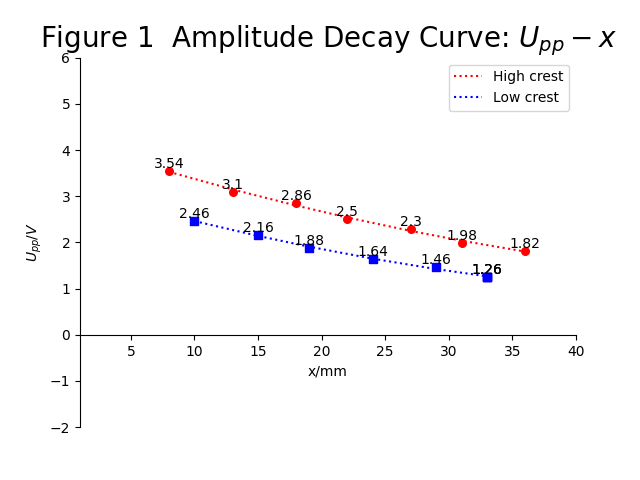
\includegraphics[width = 3in]{Figure_1.png}
  \quad
  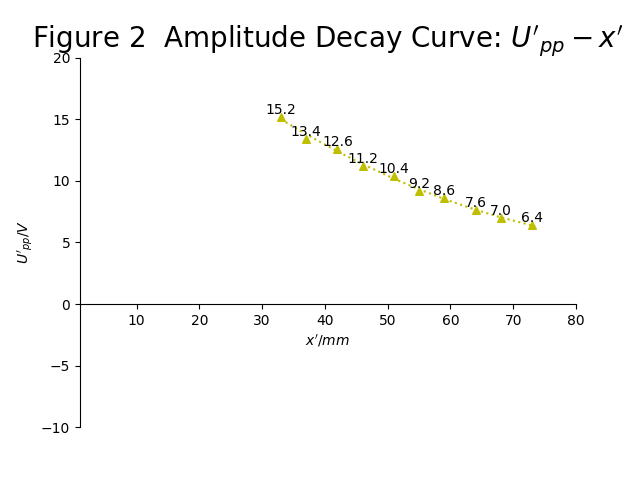
\includegraphics[width = 3in]{Figure_2.png}
\end{figure}

\begin{description}
    \item[猜想一] 声波振幅指数衰减$\quad \ln{U_{pp}} \propto x$
    \item[猜想二] 声波振幅反比例衰减$\quad U_{pp} \propto \frac1x $
    \item[猜想三] 声波振幅线性衰减$\quad U_{pp} \propto -x$
\end{description}

分别进行线性拟合(角标对应猜想中的数学模型):
\begin{description}
    \item[大峰] $r_1 = 0.9976 \quad r_2 = 0.94 \quad r_3 = 0.9956$
    \item[小峰] $r_1 = 0.9997 \quad r_2 = 0.9745 \quad r_3 = 0.994$
    \item[补充数据\footnotemark] $r_1 = 0.9987 \quad r_2 = 0.9933 \quad r_3 = 0.990$
\end{description}
\footnotetext{该组数据是另一次实验中获得,各参数与表3中不同}

对比各组相关系数,我们可以得出声波在空气中传播时最有可能以指数形式衰减,这也符合平面波与空气分子相互作用的物理图像。

\section{相位法}
\subsection{原始数据}

\begin{table}[htbp]
  \centering
  \caption{相位法数据}
    \begin{tabular}{cccccccc}
    \toprule
    i     & 1     & 2     & 3     & 4     & 5     & 6     \\
    \midrule
    $x/mm$  & 10.679 & 19.692 & 28.666 & 37.420 & 46.117 & 54.672 \\
    $x'/mm$ & 10.506 & 19.531 & 28.443 & 37.142 & 45.800 & 54.476 \\
    \bottomrule
    \end{tabular}
  \label{tab:t5}
\end{table}
声速测定仪的谐振频率为$f_0 = 40.330kHz$

\subsection{计算结果和误差分析}
最小二乘法拟合结果:
\begin{gather*}
  \Delta x = 8.7998mm \quad r = 0.99995\\
  \Delta x' = 8.7816mm \quad r' = 0.99996\\
  \Rightarrow \quad \overline{\Delta x} = 8.7907mm 
\end{gather*}

计算得
\[
    v = \overline{\Delta x} f_0 = 354.53m\cdot s^{-1}
\]

最小二乘法拟合结果随机不确定度$\frac{\sigma_k}{k} = \sqrt{\frac{1/r^2 - 1}{n - 2}}$
\[
    \Rightarrow \quad \sigma_{\Delta x} = 0.05mm \quad \sigma_{\Delta x'} = 0.04mm
\]

由不确定度传递公式
\[
    \sigma_{A \overline{\Delta x}} = \frac12 \sqrt{\sigma_{\Delta x}^2 + \sigma_{\Delta x'}^2} = 0.04mm
\]

至于波长的B类不确定度和谐振频率不确定度计算过程均与驻波法中相同,此处不再重复。

最终算得$v \pm \sigma_v = (354.5 \pm 1.7) m \cdot s^{-1}$,误差同样主要来源于最小二乘法拟合带来的随机误差。

\section{声光效应法}
\subsection{原始数据}

\begin{table}[htbp]
  \centering
  \caption{超声光栅衍射斑分布}
    \begin{tabular}{cccccccc|c}
    \toprule
    级次$k$  & -3    & -2    & -1    & 0     & 1     & 2     & 3     & 频率$f_i/MHz$ \\
    \midrule
    $x_1/cm$ & 0.00     & 2.61  & 5.23  & 7.91  & 10.55 & 13.20 & 15.85 & 9.74 \\
    $x_2/mm$ & 1.00     & 3.79  & 6.58  & 9.30  & 12.01 & 14.80 & 17.50 & 10.10 \\
    \bottomrule
    \end{tabular}
  \label{tab:t6}
\end{table}
衍射装置中光栅至场点间距$L = 639cm$,激光波长$\lambda_0 = 632.8nm$

\subsection{计算结果和误差分析}

最小二乘法拟合数据
\begin{align*}
    \Delta x_1 = 2.6446cm &\quad r_1 = 0.999995\\
    \Delta x_2 = 2.7482cm &\quad r_2 = 0.99987
\end{align*}

数据处理方法同上,取$e_L = 1cm,e_{f_i} = 0.1MHz,e_{Ax_{i}} = 0.01cm$,不考虑激光波长的不确定度,有
\[
  \frac{\sigma_{Bx_i}}{x_i} = \sqrt{\frac{1/r_i^2 - 1}{n - 2}} \Rightarrow \sigma_{Bx_1} = 0.004cm , \sigma_{Bx_2} = 0.020cm
\]

由光栅公式$d\sin{\theta} = k\lambda_0 , \theta = \frac{\Delta x_i}{L} \ll 1$,其中$d = \lambda_s$
\[
  \Rightarrow \quad v_i = \lambda_s f_i = \frac{\lambda_0 f_i L}{\overline{\Delta x_i}}
\]

算得$v_1 = 1489 m \cdot s^{-1} \quad v_2 = 1486 m \cdot s^{-1} \Rightarrow \bar{v} = 1488 m \cdot s^{-1}$
\begin{gather*}
  \sigma_v = \sqrt{(\frac{\sigma_{x_i}}{x_i})^2 + (\frac{e_L}{\sqrt3 L})^2 + (\frac{e_{f_i}}{\sqrt3 f_i})^2}\\
  \Rightarrow \quad \sigma_{v_1} = 10 m \cdot s^{-1} , \sigma_{v_2} = 14 m \cdot s^{-1}\\
  \Rightarrow \quad \sigma_{\bar{v}} = \frac{1}{2} \sqrt{\sigma_{v_1}^2 + \sigma_{v_2}^2} = 9m \cdot s^{-1}
\end{gather*}

故最终计算结果为$\bar{v} \pm \sigma_{\bar{v}} = (1488 \pm 9) m \cdot s^{-1}$

\section{驻波法补充}
在一定实验条件下,每隔0.2mm取一个数据点测定驻波振幅,绘制成图3
\begin{figure}[htb]
  \centering
  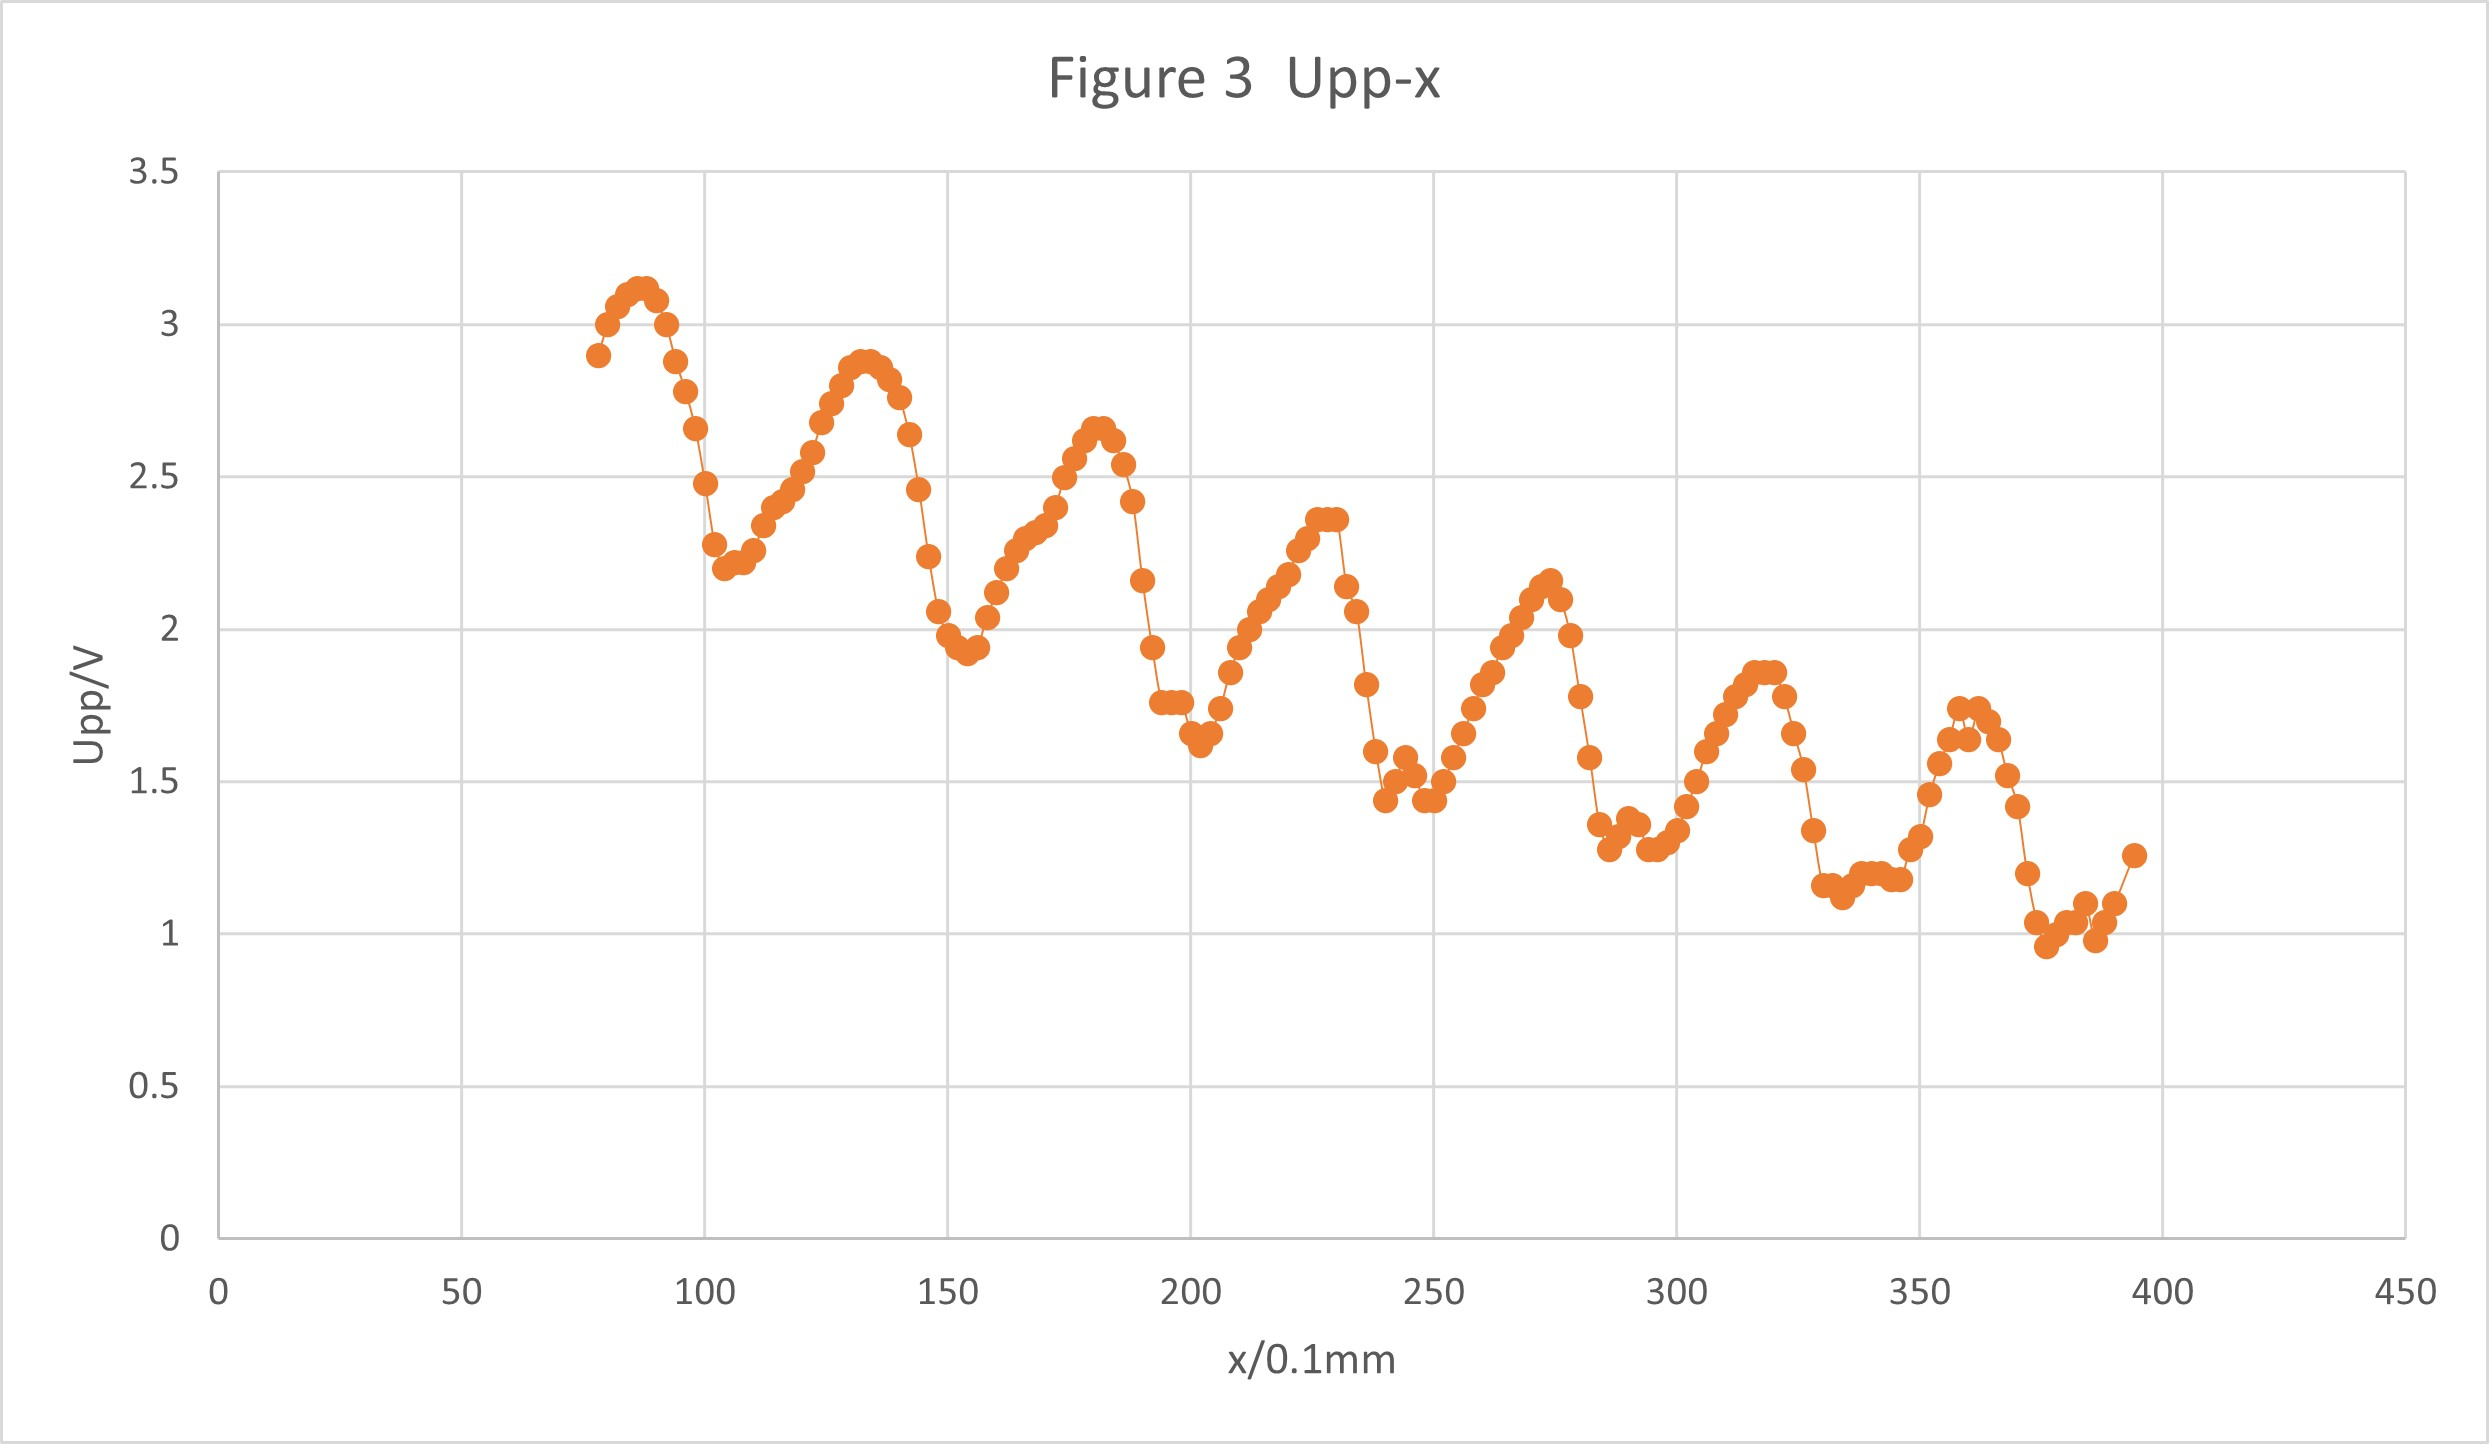
\includegraphics[width = 5in]{Figure_3.jpg}\\
  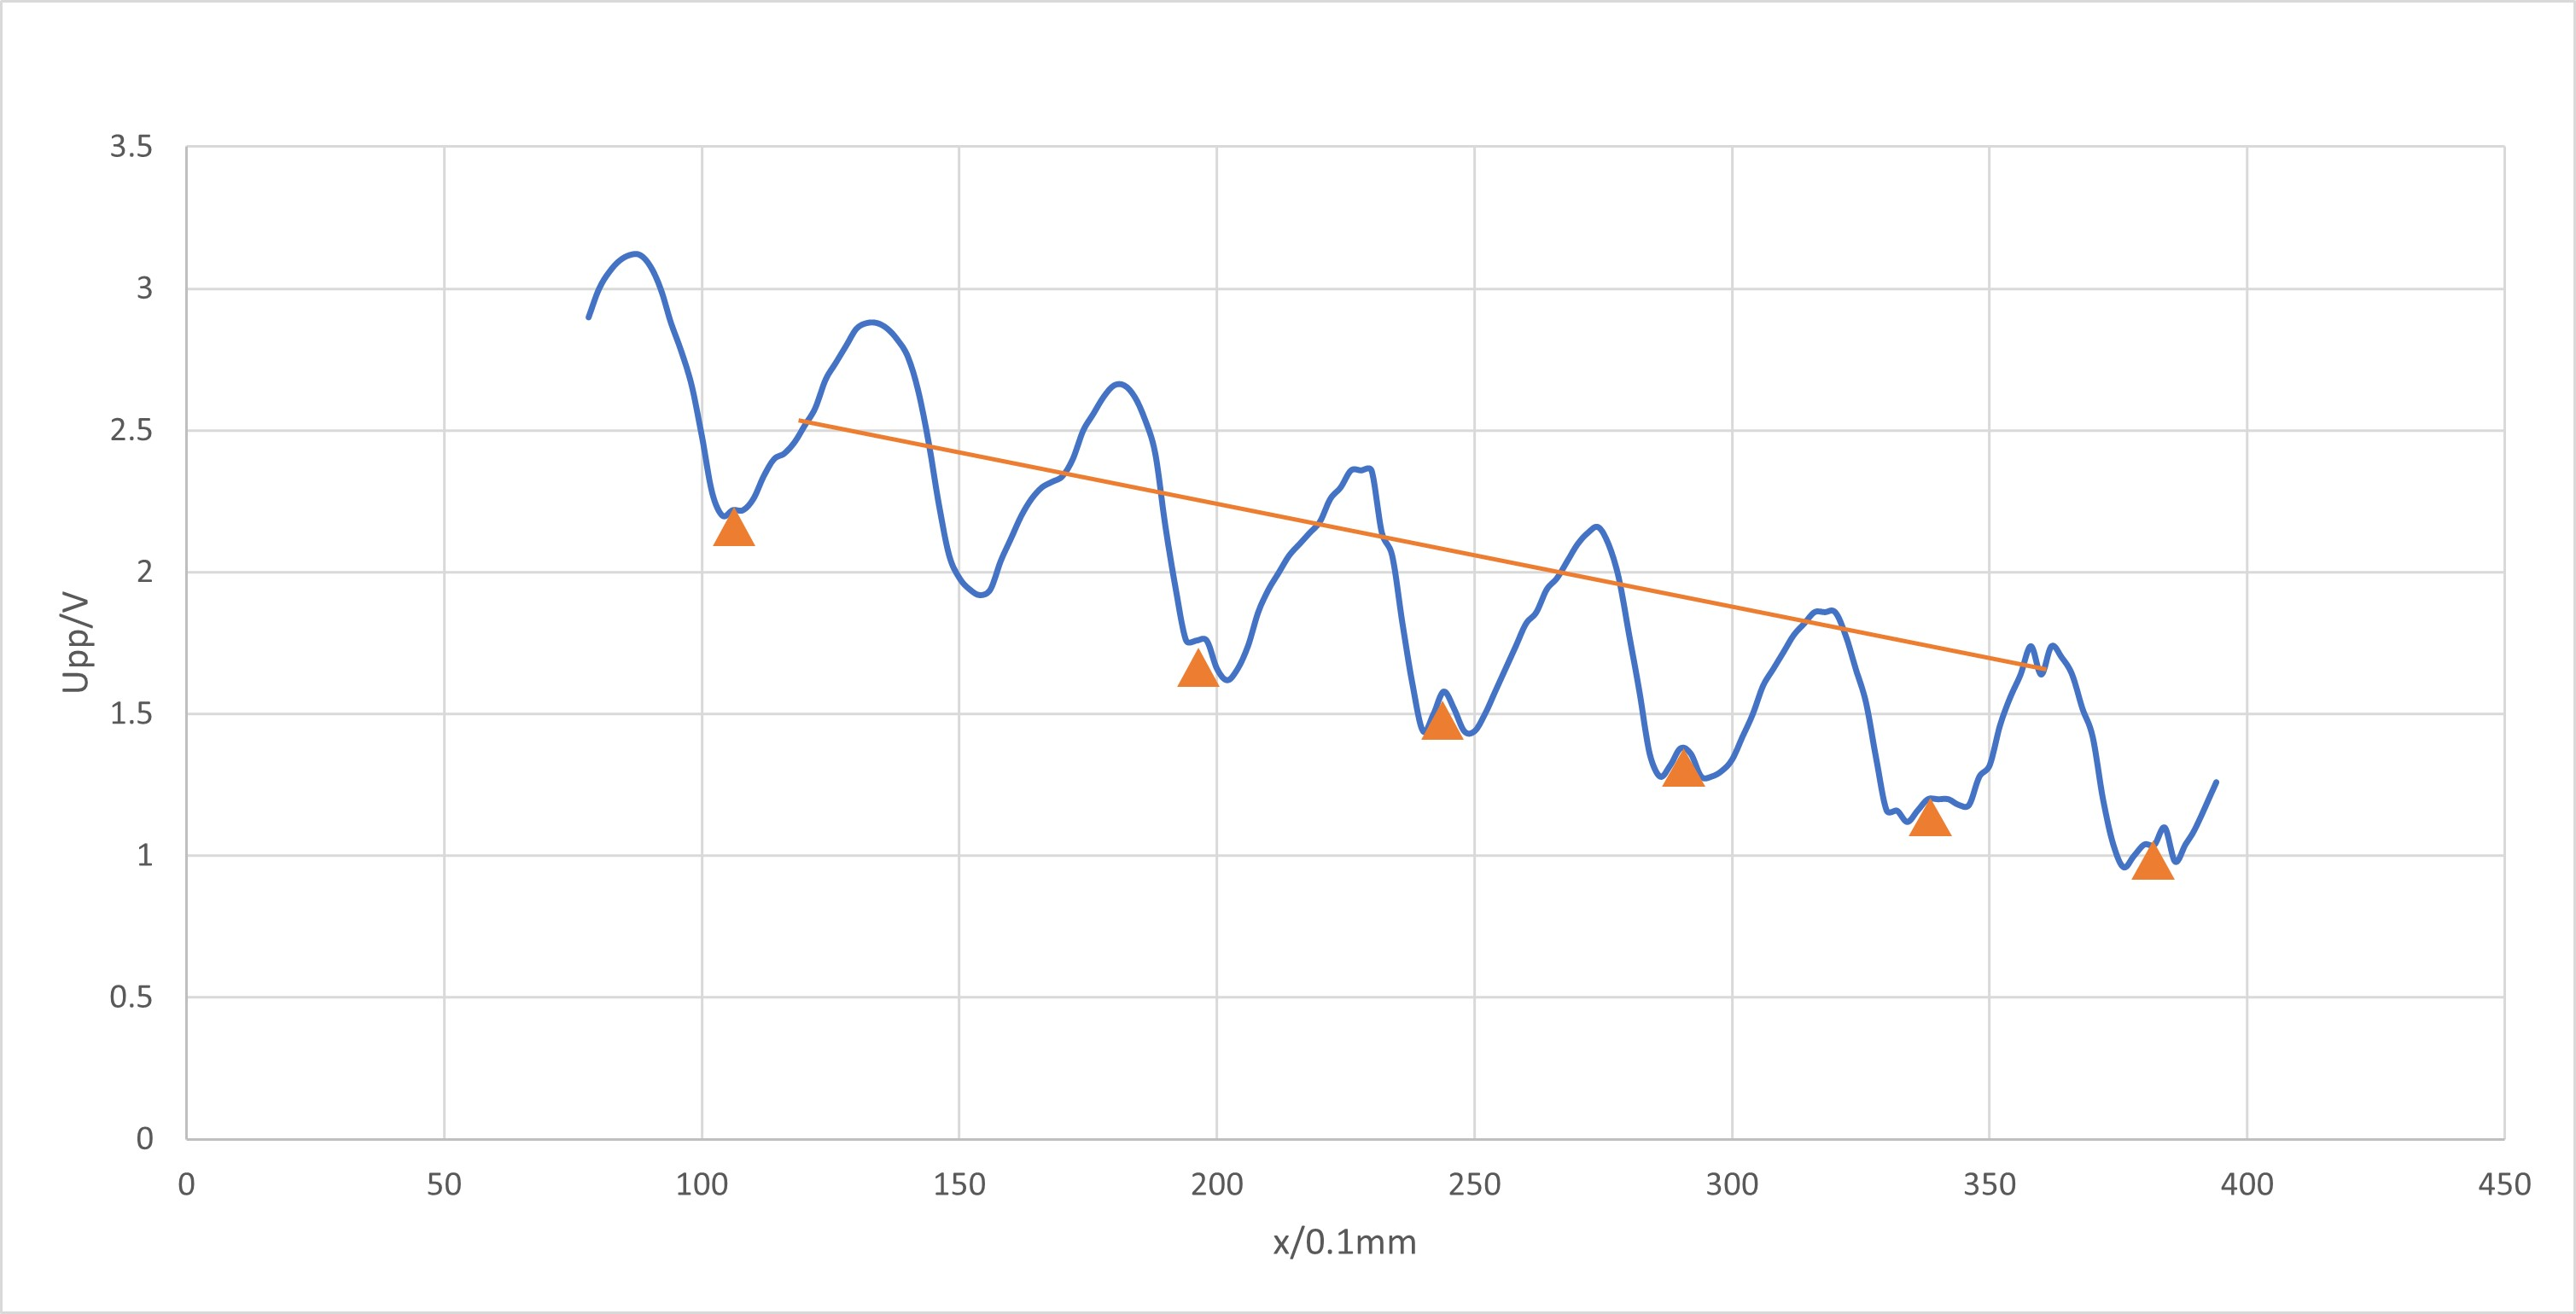
\includegraphics[width = 5in]{Figure_4.jpg}
\end{figure}

在图3中可以很明显地看出在主要的波形中存在其他的杂波干扰。
通过对主要波形上各拐点的数据分析,我们发现这些杂波具有稳定的、不同于主波形周期的周期,
且其表现出来的衰减也符合声波在空气中的衰减规律。
联系前述驻波法数据二\ref*{tab:t3}中出现的双峰现象,
我们有理由猜想在主波形之外存在一个由于实验仪器或实验环境引起的声波,
或是由于仪器内部构造使得部分声波的频率发生改变,从而显示出这一支较弱的波形。

根据对仪器的观察和数据分析,目前最可信的猜测是由于压电陶瓷换能器表面存在一层网状结构(通过观察仪器内部结构发现)
或是由于换能器的其他特性而在发射和反射声波时由于某种效应而改变了部分声波的频率,从而在示波器上显示出前述现象。

需要补充说明的一点是,在我进行测量的实验条件下,该杂波的成分占比较小,大部分情况下被主要波形掩盖,
只有在衰减到一定程度以及主波形波谷时可以较为明显地观察到。

另外存在一个问题,即在上图中出现小幅波动的情况多出现在主波振幅上升阶段,其背后又有何机理?
是一定实验条件下的偶然还是某一条件导致的必然?具体机理目前我还没有较为成熟的想法,需要进一步的理论模型推导与实验验证。

\end{document}